\section{Расчёт дальности связи.}

Используя данные моделирования, полученные в предыдущих главах, произведём оценочный расчёт дальности связи разрабатываемой системы. Структурная схема исследуемой модели показана на Рисунке \ref{fig:System-StructSch}

\begin{figure}[H]
	\centering
	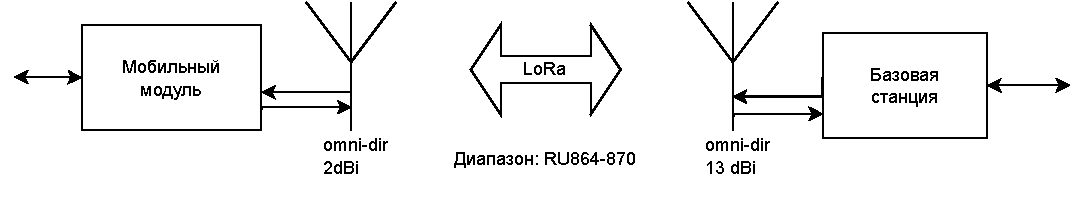
\includegraphics[width=\textwidth,keepaspectratio]{System-StructSch.pdf}
	\caption{ Структурная схема исследуемой системы}%
	\label{fig:System-StructSch}
\end{figure}

Дано:

\begin{itemize}
	\setlength\itemsep{-1ex}
	\item Усиление антенны БС – 13 дБи
	\item Усиление антенны МОУ – 2 дБи
	\item Выходная мощность – 14 дБм
	\item Чувствительность (худш) – -128 дБм
	\begin{itemize}
		\setlength\itemsep{-1ex}
		\item Бюджет канала (мин) – 142 дБ
	\end{itemize}
	\item Чувствительность (лучш) – -140 дБм
	\begin{itemize}
		\setlength\itemsep{-1ex}
		\item Бюджет канала (макс) – 154 дБ
	\end{itemize}	
\end{itemize}

Максимальная и минимальная чувствительность определяются для максимальной (11 Кб/с, SF=7) и минимальной (0.3 Кб/с, SF=12) скорости передачи данных. 

Для проведения виртуального эксперимента будем использовать модель Окамуры-Хата. Данная модель описывает процесс распространения (затухания) радиоволн в урбанизированных районах без учета информации о рельефе местности и адаптирована для расчета мобильных сетей связи. Модель Окамура-Хата предназначена для РЭС, используемых в диапазоне от 150(100) до 1 500 МГц. Модель Окамура-Хата учитывает особенности территории, застройки (городская, пригородная, открытая сельская) и населенного пункта (большой, средний, маленький).

Задача --- уложиться в предоставляемый бюджет канала. Предполагаемая высота подвеса антенны БС -- 40 м. Исследуемые высоты подвеса антенны модуля IoT -- 1-15 м. Модель потерь в городских условиях формируется следующим образом:

\begin{equation*}
	\centering
	L_U \; = \; 69.55 \; + \; 26.16 \; \lg f \; - \; 13.82 \; \lg h_B \; - \; C_H \; + \; [44.9 \; - \; 6.55 \; \lg h_B] \; \lg d
\end{equation*}

Где для небольших и средних городов:

\begin{equation*}
	\centering
	C_H \; = \; 0.8 \; + \; (\; 1.1 \; \lg f \; - \; 0.7 \; ) \; h_M \; - \; 1.56 \; \lg f 
\end{equation*}

И для больших:

\begin{equation*}
	\centering
	C_H \; = \begin{cases}\;8.29 \; (\; \lg ({1.54 h_M}))^2 \; - \; 1.1 \; \mbox{  , if } 150 \le f \le 200 \\ \; 3.2 \; (\lg ({11.75 h_M}))^2 \; - \; 4.97 \; \mbox{ , if }200 < f \le 1500 \end{cases}
\end{equation*}

Здесь:
$L_U$ — потери в городских условиях, дБ
$h_B$ — высота подвеса базовой антенны
$h_M$ — высота подвеса мобильной антенны
$f$ — частота передачи
$C_H$ — коэффициент коррекции антенны
$d$  — дистанция связи

Потери в условиях пригорода рассчитываются по формуле:

\begin{equation*}
	\centering
	L_{SU}\; = \; L_U \; - \; 2 \big( \lg {\frac{f}{28}}\big)^2 \; - \;5.4 
\end{equation*}

И, наконец, в открытых условиях:

\begin{equation*}
	\centering
	L_{O}\; = \; L_U \; - \; 4.78 \big( \lg {f}\big)^2 \; + \; 18.33 \big( \lg {f}\big)- \;40.94
\end{equation*}
 
Расчеты будем вести в MATLAB. Листинг кода представлен в Приложении A. 

Результаты расчёта показаны на Рисунках \ref{fig:system-count-city} и \ref{fig:system-count-suburb}. Ось oY показывает уровень потерь, ось oX показывает расстояние между устройствами. Горизонтальная черта показывает уровень потерь, при превышении которого количество ошибок будет превышать 1\%.


\begin{figure}[H]
	\centering
	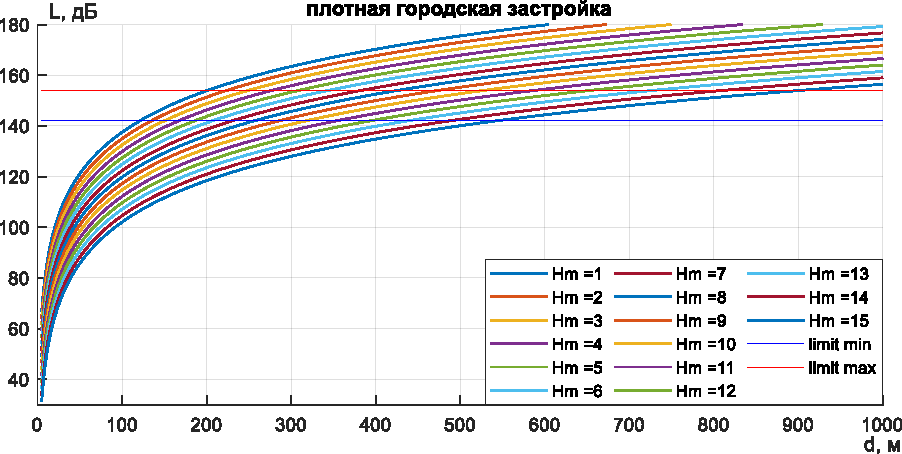
\includegraphics[width=\textwidth,keepaspectratio]{system-count-city.pdf}
	\caption{Результаты расчёта дальности связи в условиях плотной городской застройки.}
	\label{fig:system-count-city}
\end{figure}

\begin{figure}[H]
\centering
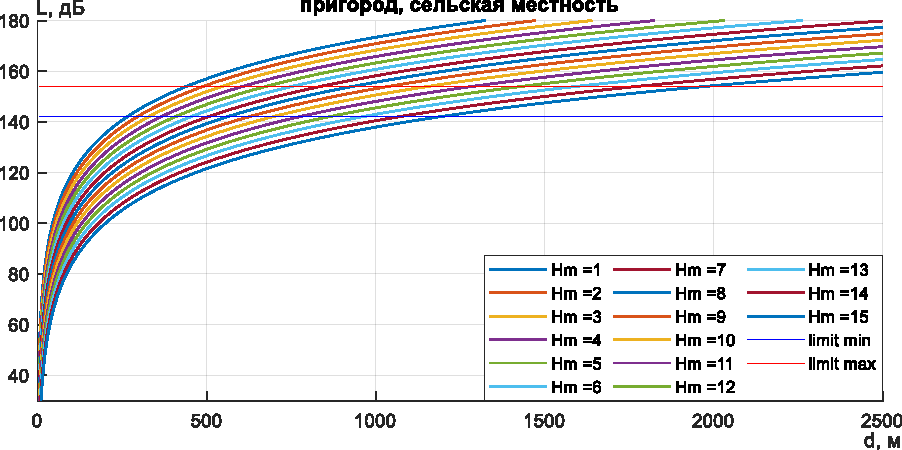
\includegraphics[width=\textwidth,keepaspectratio]{system-count-suburb.pdf}
\caption{Результаты расчёта дальности связи в условиях пригорода и сельской местности.}
\label{fig:system-count-suburb}
\end{figure}

Проведённые расчеты позволяют приблизительно оценить структуру сети, а следовательно проводить предварительные экономические расчеты.




